\documentclass[10pt,twocolumn]{article}
\usepackage[margin=0.9in]{geometry}
\usepackage{graphicx}
\usepackage{hyperref}
\usepackage{cite}


\title{\large{Spectral Clustring Based on Local PCA with Application to Hand-written Digit Separation}}
\author{
    Yu, Guangting\thanks{Quantitative Finance \& Risk Management, Department of Mathematics} \\
    \small{\texttt{yugtmath@umich.edu}}
    \and
    Jia, Guo\thanks{Applied \& Interdisciplinary Math Ph.D., Department of Mathematics} \\
    \texttt{guojia@umich.edu}
    \and
    Tsukamoto, Masaya\thanks{Quantitative Finance \& Risk Management, Department of Mathematics} \\
    \texttt{masayats@umich.edu}
    \and
    Wang, Zihan\thanks{Space Science Ph.D., Department of Climate and Space Sciences and Engineering} \\
    \texttt{wzihan@umich.edu}
}


\begin{document}
\maketitle

\subsection*{Problem statement}
\begin{figure}[htbp]
\centering

\includegraphics[width=0.1\textwidth]{connected-digits.png}
\hspace{1em}
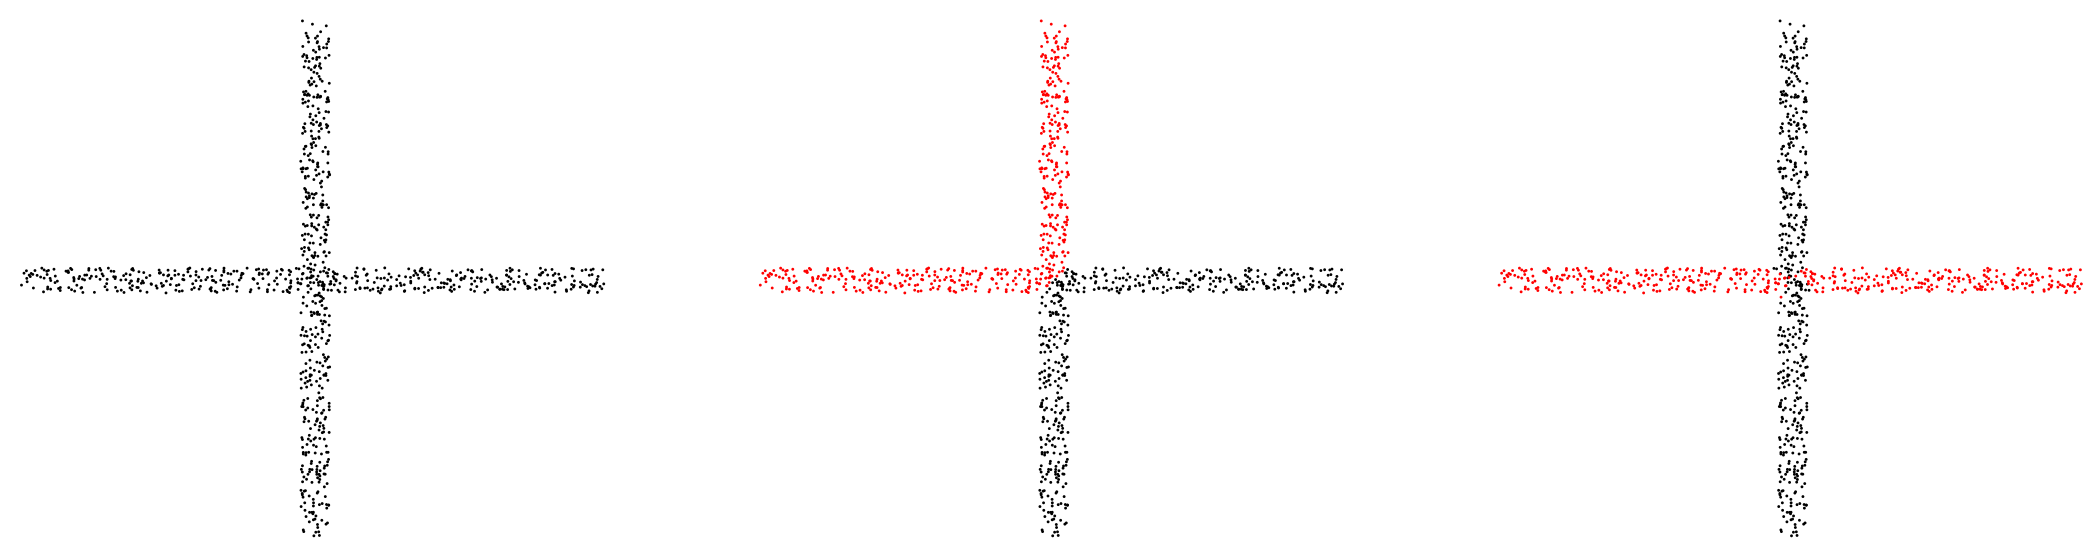
\includegraphics[width=0.3\textwidth]{effect.png}
\caption{(1) Connected digits, (2) sample pixels (3) spectral clustering by Ng. et al (2002), (4) spectral clustering by local PCA}
\label{fig1}
\end{figure}
In hand-written digit recognition, if the digits are connected, (like `2' and `0' in Figure \ref{fig1}), there is no chance for the classifier to output the correct result.
So we want to separate the connected digits apart.
\subsection*{Motivation}
This problem is motivated from one of the computer vision problem to recognize hand-written digits.
Many good algorithms have been developed to classify a single digit with very high accuracy.
However, when we switch to multiple digits, one of the difficulty occurs is that if the digits are accidentally connected, 
\subsection*{Papers to focus on}
Paper 


\href{http://www.jmlr.org/papers/volume18/14-318/14-318.pdf}{(Arias-Castro and Lerman, Zhang,2017)}
\href{https://papers.nips.cc/paper/4246-sparse-manifold-clustering-and-embedding.pdf}{(Elhamifar and Vidal, 2011)}
\href{http://sciences.ucf.edu/math/tengz/wp-content/uploads/sites/45/2016/07/code.zip}{code}
\cite{Arias-Castro:2017:SCB:3122009.3122018}
\subsection*{Methods to be compared}
\subsection*{Data sets}
\subsection*{Group member roles}

\newpage
\bibliography{reference}{}
\bibliographystyle{plain}
\end{document}